No fue posible modificar o alterar la interacción con el servidor de Waze dado que el protocolo está ofuscado y no podemos realizar auditoría al respecto. 
\\\\
De todas formas, se alteró el comportamiento de la conectividad de Waze  utilizando IPTables para ver su comportamiento.
\\\\    
Con IPTables, al momento de realizar una petición de rutas en Waze (colocando una dirección a la cual queremos llegar), añadimos una regla que votara todo tráfico proveniente que tuviera la IP con la cual nuestra APP se había estado comunicando:
\\\\
iptables -A INPUT -s 65.55.44.100 -j DROP
\\\\
Estos argumentos en IPTables indican que debe ser añadida una regla para los paquetes de entrada (INPUT) desde el origen (-s) 65.55.33.100 con la acción DROP (votar el paquete).

            \begin{figure}[H]
  \begin{center}
    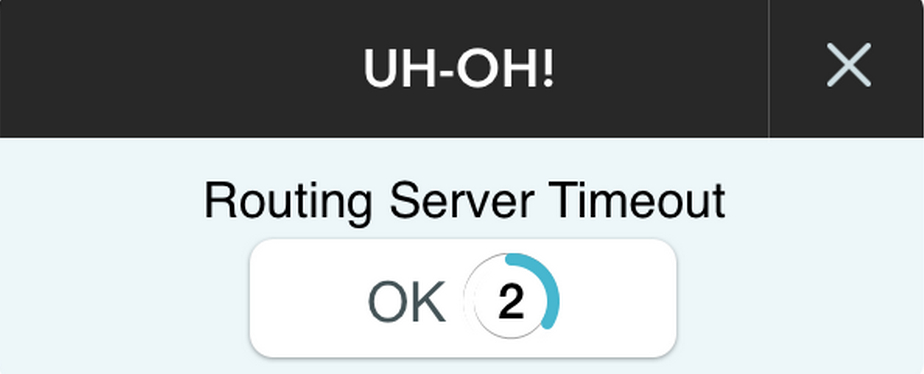
\includegraphics[width=0.3\textwidth]{imagenes/fig45.png}
    \caption{Error de conexión a internet}
  \end{center}
\end{figure}
    
    
Waze al no recibir los paquetes de respuesta de la solicitud de ruteo nos advierte que esperó al servidor de rutas pero este no le respondió [Figura 17].
\\\\
De manera similar, se hizo para cuando se hizo una alerta de tráfico en Waze, al seleccionar que había mucho tráfico en nuestra ubicación, se realizó el mismo comando con IPTables.

        \begin{figure}[H]
  \begin{center}
    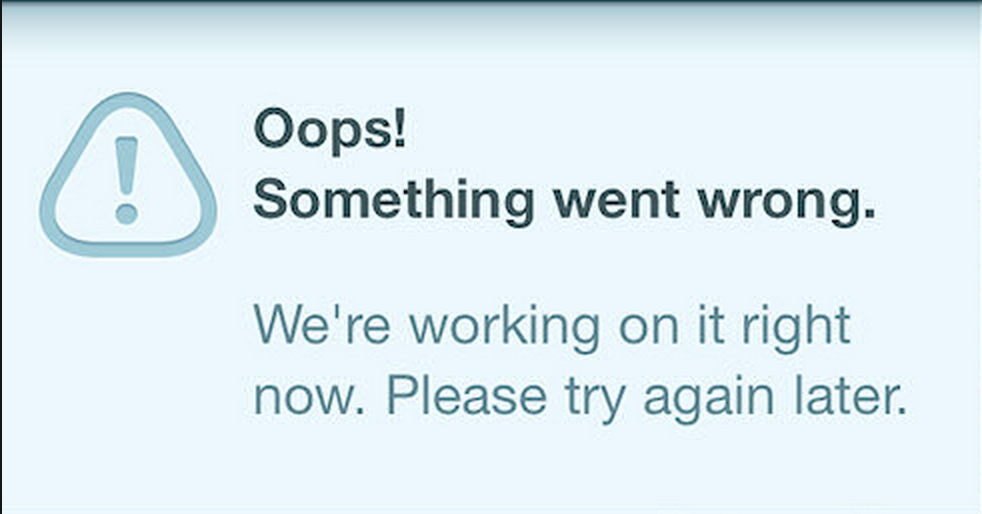
\includegraphics[width=0.3\textwidth]{imagenes/fig46.png}
    \caption{Error generado al ser modificado previamente un servidor DNS en el dispositivo}
  \end{center}
\end{figure}


Waze nos advierte que hay un error, pero esta vez no nos indica de qué se trata. Podría ser una excepción no rescatada dentro del código (Figura[18]).
